% Created 2025-08-04 Mon 00:40
% Intended LaTeX compiler: pdflatex
\documentclass[11pt]{article}
\usepackage[utf8]{inputenc}
\usepackage[T1]{fontenc}
\usepackage{graphicx}
\usepackage{longtable}
\usepackage{wrapfig}
\usepackage{rotating}
\usepackage[normalem]{ulem}
\usepackage{amsmath}
\usepackage{amssymb}
\usepackage{capt-of}
\usepackage{hyperref}
\author{Felipe Merino y Uriel Dueñas}
\date{2025-07-30}
\title{Proyecto ICCD332 Arquitectura de Computadores}
\hypersetup{
 pdfauthor={Felipe Merino y Uriel Dueñas},
 pdftitle={Proyecto ICCD332 Arquitectura de Computadores},
 pdfkeywords={},
 pdfsubject={},
 pdfcreator={Emacs 27.1 (Org mode 9.7.5)}, 
 pdflang={Spanish}}
\begin{document}

\maketitle
\tableofcontents

\section{City Weather APP}
\label{sec:org50d0b09}
\subsection{Conocimientos adquiridos:}
\label{sec:orgd7e9484}

\begin{enumerate}
\item Conocimientos de sistema operativo Linux
\item Conocimientos de Emacs/Jupyter
\item Configuración de Entorno para Data Science con Mamba/Anaconda
\item Literate Programming
\end{enumerate}

\subsection{Estructura del proyecto}
\label{sec:org8e10f9c}

Estructura final de las carpetas de nuestro proyecto:

\begin{verbatim}
.
├── CityTemperatureAnalysis1.ipynb
├── CityTemperatureAnalysis1.ipynb:Zone.Identifier
├── Cohete.zip:Zone.Identifier
├── LICENSE
├── README.md
├── climaMelbourne.csv
├── get-weather.sh
├── get-weather.sh:Zone.Identifier
├── get-weather.sh~
├── main.py
├── main.py:Zone.Identifier
├── output.log
└── weather-site
    ├── Org-Website.org
    ├── Org-Website.org:Zone.Identifier
    ├── build-site.el
    ├── build.sh
    ├── content
    │   ├── images
    │   ├── index.org
    │   ├── index.org:Zone.Identifier
    │   └── index.org~
    └── public
        ├── images
        └── index.html

6 directories, 20 files
\end{verbatim}

\section{Formulación del Problema y Objetivos}
\label{sec:orgac53fc9}

\textbf{\textbf{Problema:}}
Se desea realizar un registro climatológico de una ciudad
\(\mathcal{C}\). Para esto, escriba un script de Python/Java que permita
obtener datos climatológicos desde el API de \href{https://openweathermap.org/current\#one}{openweathermap}. El API
hace uso de los valores de latitud \(x\) y longitud \(y\) de la ciudad
\(\mathcal{C}\) para devolver los valores actuales a un tiempo \(t\).



\section{Metodología y Herramientas}
\label{sec:orge27fc2b}

El proyecto se desarrolló siguiendo estos pasos:

\begin{enumerate}
\item \textbf{Obtención de Credenciales}: Se generó una clave de API gratuita en el portal de \href{https://openweathermap.org/current\#one}{OpenWeatherMap}.
\item \textbf{Desarrollo del Script}: Se codificó el script main.py para gestionar las
solicitudes al API y el almacenamiento de datos
\item \textbf{Automatización}: Se configuró el entorno de ejecución con el archivo \texttt{get-weather.sh} y
se programó su ejecución con Crontab
\item \textbf{Análisis de Datos}: Se utilizaron las librerías Pandas y Matplotlib para procesar
y visualizar la información.
\end{enumerate}

Las herramientas clave utilizadas fueron:
\begin{itemize}
\item \textbf{Lenguaje de Programación}: Python 3
\item \textbf{Librerías}: Requests, Pandas, Matplotlib.
\item \textbf{Entorno}: Mamba/Conda sobre Linux (WSL)
\item \textbf{Automatización}: Shell scripting y Crontab
\item \textbf{Documentación}: Emacs Org Mode
\end{itemize}

\section{Desarrollo e Implementación}
\label{sec:org7fe217b}
\subsection{Script de Python (\texttt{main.py})}
\label{sec:org47747b3}

El corazón del proyecto es un script de Python que realiza tres tareas principales:
\begin{enumerate}
\item \textbf{Consulta al API}: Llama al endpoint de OpenWeatherMap para obtener datos
\item \textbf{Verificación de Alertas}: Revisa los datos recibidos para detectar condiciones climáticas
extremas
\item \textbf{Escritura en CSV}: Almacena los datos relevantes en un archivo \texttt{climaMelbourne.csv},
añadiendo una nueva fila en cada ejecución sin borrar las anteriores
\end{enumerate}

\begin{verbatim}
import csv
import datetime

import requests



LAT = -37.813061
LONGITUDE = 144.944214
API_KEY = "d342e18efa48c85976dbaa3493b34dd4"
FILE_NAME = "climaMelbourne.csv"
BASE_URL = "http://api.openweathermap.org/data/2.5/weather"

# https://iabigdata-soka-4ae9e223e32444ac5ae3d78afbd55fd9aa6da1c19d9679bf.gitlab.io/post/2024-06-06-pia_openweathermap_ex/#:~:text=Este%20sistema%20consulta%20la%20API,clim%C3%A1ticos%20de%20diferentes%20ubicaciones%20y


def get_weather(lat, lon):
    url = f"http://api.openweathermap.org/data/2.5/weather?lat={lat}&lon={lon}&appid={API_KEY}&units=metric&lang=es"
    try:
        response = requests.get(url)
        response.raise_for_status()
        return response.json()
    except Exception as e:
        print("Error al obtener clima:", e)
        return None


def verificar_alertas(data):
    alertas = []  # Lista para almacenar alertas

    # Verifica si la temperatura supera los 35°C
    if data["main"]["temp"] > 35:
        alertas.append("Alerta de calor extremo")

    # Verifica si la velocidad del viento supera los 20 m/s
    if data["wind"]["speed"] > 20:
        alertas.append("Alerta de viento fuerte")

    # Segun entendi pidio para eso, estaba en el json de la pagina para esas horas
    # Verifica si hay datos de lluvia
    """if "rain" in data and ("1h" in data["rain"]):
        alertas.append("Alerta de lluvia")"""
    if "rain" in data and data["rain"].get("1h", 0) > 0:
        alertas.append("Alerta de lluvia")

    # Verificar nieve
    """if "snow" in data and ("1h" in data["snow"]):
        alertas.append("Alerta de nieve")"""
    if "snow" in data and data["snow"].get("1h", 0) > 0:
        alertas.append("Alerta de nieve")

    return alertas


# https://www.geeksforgeeks.org/python/python-find-current-weather-of-any-city-using-openweathermap-api/


def writeCSV(data, alertas):
    # Encabezados para el archivo CSV
    campos = [
        "ciudad",
        "lat",
        "lon",
        "temp",
        "humedad",
        "viento",
        "description",
        "lluvia",
        "nieve",
        "fecha",
        "alertas",
    ]

    # Crear archivo con encabezado si aún no existe
    try:
        with open(FILE_NAME, mode="x", newline="") as file:
            writer = csv.writer(file)
            writer.writerow(campos)
    except FileExistsError:
        pass

    # Agregar los datos y alertas en una nueva fila del archivo
    with open(FILE_NAME, mode="a", newline="") as file:
        writer = csv.writer(file)
        writer.writerow(
            [
                data["name"],
                LAT,
                LONGITUDE,
                data["main"]["temp"],
                data["main"]["humidity"],
                data["wind"]["speed"],
                data["weather"][0]["description"],
                data.get("rain", {}).get("1h", 0),
                data.get("snow", {}).get("1h", 0),
                datetime.datetime.now().strftime("%Y-%m-%d %H:%M:%S"),
                "; ".join(alertas),
            ]
        )


def main():
    print("===== Clima Melbourne =====")
    melbourne_weather = get_weather(LAT, LONGITUDE)
    if melbourne_weather and melbourne_weather.get("cod") == 200:
        alertas = verificar_alertas(melbourne_weather)
        writeCSV(melbourne_weather, alertas)
        print(f"Datos guardados para {melbourne_weather['name']}")
        if alertas:
            print("Alertas activadas:", ", ".join(alertas))
    else:
        print("Error: Ciudad no disponible o API KEY inválida")


if __name__ == "__main__":
    main()
\end{verbatim}
\captionof{figure}{Archivo main.py}


\subsection{Script de Automatización (\texttt{get-weather.sh})}
\label{sec:org7bf1633}

Para asegurar que el script de Python se ejecute en el entorno de Conda correcto, creamos un script de shell. Este script activa el entorno \texttt{iccd332} y luego ejecuta \texttt{main.py}.

\begin{verbatim}
===== Clima Melbourne =====
Datos guardados para Melbourne
\end{verbatim}



Para darle los respectivos permisos de ejecución al archivo se usó:

\subsection{Configuración de Crontab}
\label{sec:org92608b3}

La automatización final se logra con \texttt{crontab}, el programador de tareas de Linux
Se configuró una tarea para ejecutar \texttt{get-weather.sh} cada 4 minutos.
La salida y los errores se redirigen al archivo \texttt{output.log} para su posterior revisión


Para configurar se utiliza el comando:
verificamos si se guardó con el comando:

\begin{verbatim}
*/4 * * * * cd /home/iccd332/org-ProyectoFinal && ./get-weather.sh >> output.log 2>&1
\end{verbatim}


Cada asterisco de: * /4 * * * *
Representa:
\begin{itemize}
\item Minutos (en este caso 4)
\begin{itemize}
\item hora
\begin{itemize}
\item día del mes
\begin{itemize}
\item mes
\begin{itemize}
\item día de la semana
\end{itemize}
\end{itemize}
\end{itemize}
\end{itemize}
\end{itemize}
cd /home/iccd332/org-ProyectoFinal \&\& ./get-weather.sh

se moverá en el directorio y ejecutará el archivo get-weather.sh

>> output.log 2>\&

Se encarga de guardar toda salida que de el programa en el archivo output.log


Finalmente, hacemos los cambios en el sitio web con:
y lo mostramos con:
\section{Análisis y Visualización de Resultados}
\label{sec:orga842572}

\subsection{Carga de Datos y Muestra}
\label{sec:orgc98d313}

Primero, cargamos el archivo \texttt{climaMelbourne.csv} en un DataFrame de Pandas para facilitar su manipulación.

\begin{verbatim}
import pandas as pd

# Lectura del archivo CSV de Melbourne con la ruta absoluta
df = pd.read_csv('/home/iccd332/org-ProyectoFinal/climaMelbourne.csv')

# Se imprime la estructura del DataFrame (filas x columnas)
print(df.shape)
\end{verbatim}
\captionof{figure}{Carga de datos y verificación de dimensiones}

\begin{verbatim}
(59, 11)
\end{verbatim}


A continuación, mostramos una muestra aleatoria de 10 registros para observar la estructura y variedad de los datos.

\begin{verbatim}
# --- INSTRUCCIÓN ---
from tabulate import tabulate

sample_df = df.sample(10)
org_table_string = tabulate(sample_df, headers='keys', tablefmt='orgtbl')

# Guardar la tabla formateada en un archivo temporal
with open("/tmp/org_table.txt", "w") as f:
    f.write(org_table_string)
\end{verbatim}
\captionof{figure}{Generar muestra y guardar en archivo temporal}


\begin{verbatim}
# Ejecuto un archivo temporal creado con los datos del DataFrame
cat /tmp/org_table.txt
\end{verbatim}
\captionof{figure}{Muestra aleatoria de 10 registros del DataFrame}

\begin{center}
\begin{tabular}{rlrrrrrlrrlr}
 & ciudad & lat & lon & temp & humedad & viento & description & lluvia & nieve & fecha & alertas\\[0pt]
\hline
21 & Melbourne & -37.8131 & 144.944 & 17.34 & 61 & 4.47 & muy nuboso & 0 & 0 & 2025-08-03 22:04:05 & nan\\[0pt]
20 & Melbourne & -37.8131 & 144.944 & 17.3 & 62 & 3.13 & muy nuboso & 0 & 0 & 2025-08-03 22:00:05 & nan\\[0pt]
36 & Melbourne & -37.8131 & 144.944 & 17.83 & 60 & 3.58 & muy nuboso & 0 & 0 & 2025-08-03 23:04:05 & nan\\[0pt]
39 & Melbourne & -37.8131 & 144.944 & 17.84 & 59 & 4.92 & muy nuboso & 0 & 0 & 2025-08-03 23:16:06 & nan\\[0pt]
29 & Melbourne & -37.8131 & 144.944 & 17.64 & 60 & 10.29 & muy nuboso & 0 & 0 & 2025-08-03 22:36:08 & nan\\[0pt]
6 & Melbourne & -37.8131 & 144.944 & 16.65 & 63 & 4.47 & muy nuboso & 0 & 0 & 2025-08-03 21:04:15 & nan\\[0pt]
15 & Melbourne & -37.8131 & 144.944 & 16.99 & 62 & 3.13 & muy nuboso & 0 & 0 & 2025-08-03 21:40:05 & nan\\[0pt]
37 & Melbourne & -37.8131 & 144.944 & 17.83 & 60 & 3.58 & muy nuboso & 0 & 0 & 2025-08-03 23:08:07 & nan\\[0pt]
24 & Melbourne & -37.8131 & 144.944 & 17.35 & 61 & 4.02 & muy nuboso & 0 & 0 & 2025-08-03 22:16:08 & nan\\[0pt]
41 & Melbourne & -37.8131 & 144.944 & 17.83 & 60 & 4.02 & muy nuboso & 0 & 0 & 2025-08-03 23:24:07 & nan\\[0pt]
\end{tabular}
\end{center}

\subsection{Gráfica de Temperatura vs. Tiempo}
\label{sec:orgcd68173}

Esta gráfica muestra la fluctuación de la temperatura a lo largo del tiempo.

\begin{verbatim}
import matplotlib.pyplot as plt
import matplotlib.dates as mdates
import pandas as pd

df['fecha'] = pd.to_datetime(df['fecha'])

# Define el tamaño de la figura de salida
fig, ax = plt.subplots(figsize=(10, 6))

# Dibuja las variables fecha y temp
ax.plot(df['fecha'], df['temp'], marker='.', linestyle='-', color='orangered')

# ajuste para presentacion de fechas en la imagen
ax.xaxis.set_major_locator(mdates.HourLocator(interval=6))
ax.xaxis.set_major_formatter(mdates.DateFormatter('%d-%b %H:%M'))

ax.grid(True, linestyle='--', alpha=0.6)

# Titulo que obtiene el nombre de la ciudad del DataFrame
plt.title(f'Temperatura vs. Tiempo en {df["ciudad"].iloc[0]}')
plt.xlabel('Fecha y Hora')
plt.ylabel('Temperatura (°C)')

# rotación de las etiquetas 45°
plt.xticks(rotation=45)
fig.tight_layout()

fname = './images/temperature_melbourne.png'
plt.savefig(fname)
fname
\end{verbatim}
\captionof{figure}{Gráfica de Temperatura vs. Tiempo en Melbourne}

\begin{center}
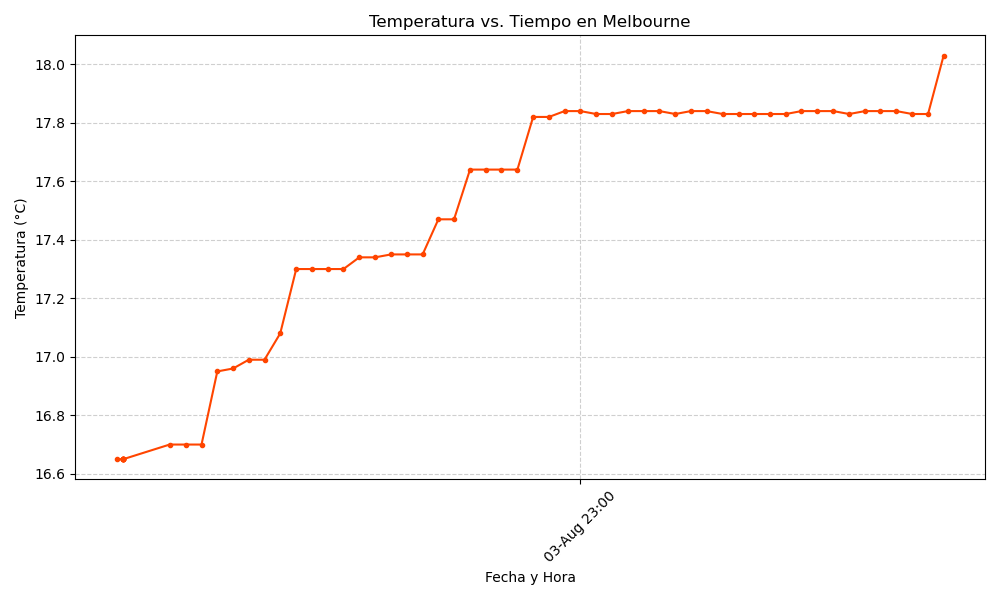
\includegraphics[width=.9\linewidth]{./images/temperature_melbourne.png}
\end{center}

Como el servidor http de emacs se ejecuta desde la carpeta public
es necesario copiar el archivo a la ubicacion public/images

\begin{verbatim}
cp -rfv ./images/* ../public/images/
\end{verbatim}

\subsection{Gráfica de Humedad con respecto al tiempo}
\label{sec:orgcc60fdb}

\begin{verbatim}
import matplotlib.pyplot as plt
import matplotlib.dates as mdates
import pandas as pd

df['fecha'] = pd.to_datetime(df['fecha'])

# Define el tamaño de la figura de salida
fig, ax = plt.subplots(figsize=(10, 6))

# Dibuja las variables fecha y humedad
ax.plot(df['fecha'], df['humedad'], marker='.', linestyle='-', color='dodgerblue')

# ajuste para presentacion de fechas en la imagen
ax.xaxis.set_major_locator(mdates.HourLocator(interval=6))
ax.xaxis.set_major_formatter(mdates.DateFormatter('%d-%b %H:%M'))

ax.grid(True, linestyle='--', alpha=0.6)

# Titulo que obtiene el nombre de la ciudad del DataFrame
plt.title(f'Humedad vs. Tiempo en {df["ciudad"].iloc[0]}')
plt.xlabel('Fecha y Hora')
plt.ylabel('Humedad Relativa (%)')

# rotación de las etiquetas 45°
plt.xticks(rotation=45)
fig.tight_layout()

fname = './images/humidity_melbourne.png'
plt.savefig(fname)
fname
\end{verbatim}
\captionof{figure}{Gráfica de Humedad (\%) vs. Tiempo en Melbourne.}

\begin{center}
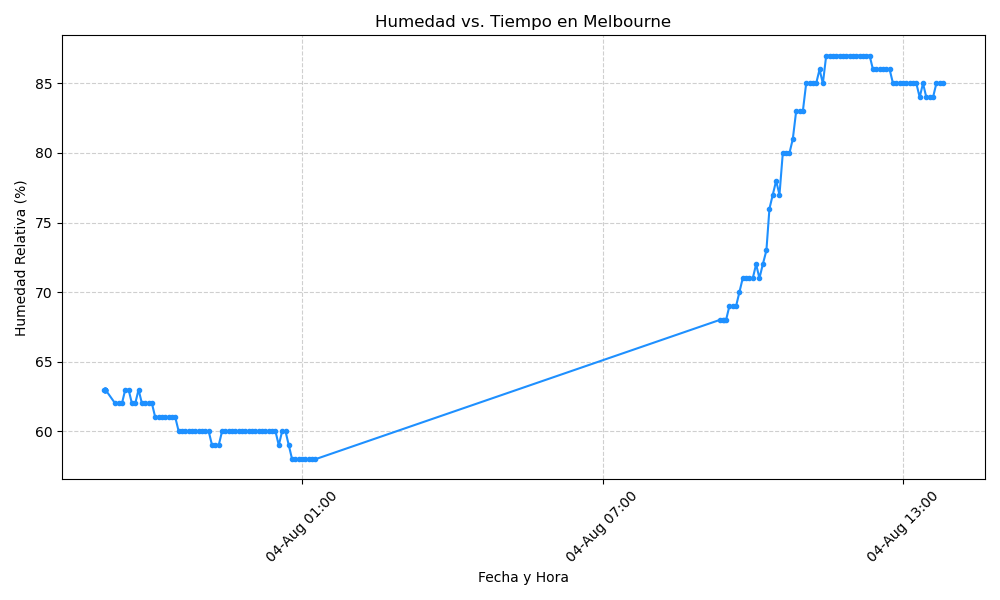
\includegraphics[width=.9\linewidth]{./images/humidity_melbourne.png}
\end{center}

\begin{verbatim}
cp -rfv ./images/* ../public/images/
\end{verbatim}


\subsection{Gráfica de Velocidad del Viento con respecto al tiempo}
\label{sec:orgec24f17}

\begin{verbatim}
import matplotlib.pyplot as plt
import matplotlib.dates as mdates
import pandas as pd

df['fecha'] = pd.to_datetime(df['fecha'])

# Define el tamaño de la figura de salida
fig, ax = plt.subplots(figsize=(10, 6))

# Dibuja las variables fecha y viento
ax.plot(df['fecha'], df['viento'], marker='.', linestyle='-', color='seagreen')

# ajuste para presentacion de fechas en la imagen
ax.xaxis.set_major_locator(mdates.HourLocator(interval=6))
ax.xaxis.set_major_formatter(mdates.DateFormatter('%d-%b %H:%M'))

ax.grid(True, linestyle='--', alpha=0.6)

# Titulo que obtiene el nombre de la ciudad del DataFrame
plt.title(f'Velocidad del Viento vs. Tiempo en {df["ciudad"].iloc[0]}')
plt.xlabel('Fecha y Hora')
plt.ylabel('Viento (m/s)')

# rotación de las etiquetas 45°
plt.xticks(rotation=45)
fig.tight_layout()

fname = './images/wind_melbourne.png'
plt.savefig(fname)
fname
\end{verbatim}
\captionof{figure}{Gráfica de Velocidad del Viento (m/s) vs. Tiempo en Melbourne.}

\begin{center}
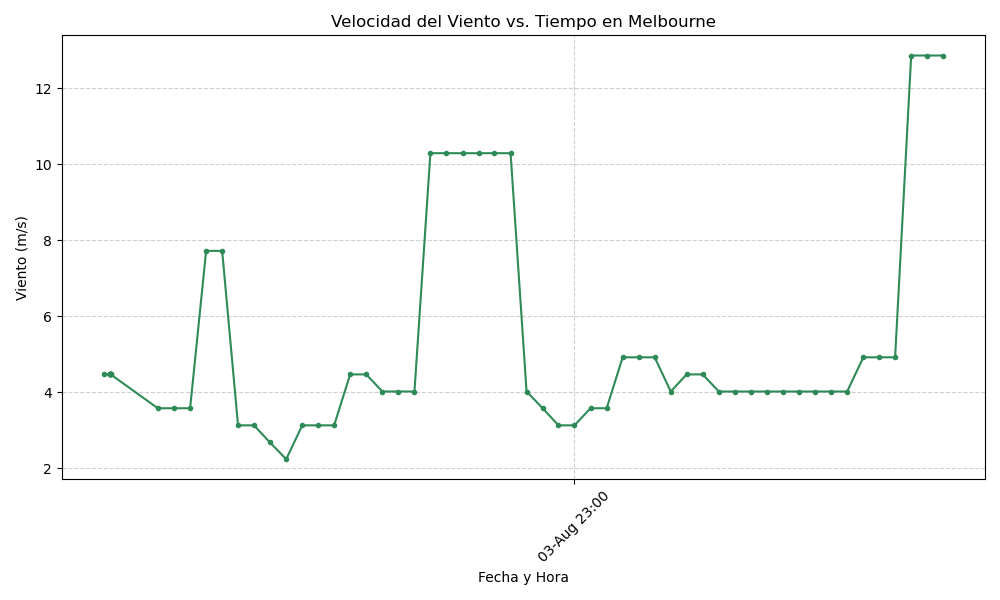
\includegraphics[width=.9\linewidth]{./images/wind_melbourne.png}
\end{center}

\begin{verbatim}
cp -rfv ./images/* ../public/images/
\end{verbatim}

\section{Referencias}
\label{sec:org76e6d33}
\begin{itemize}
\item \href{https://emacs.stackexchange.com/questions/28715/get-pandas-data-frame-as-a-table-in-org-babel}{Presentar DataFrame como tabla en Emacs Org}
\item \href{https://orgmode.org/worg/org-contrib/babel/languages/ob-doc-python.html}{Python Source Code Blocks in Org Mode}
\item \href{https://systemcrafters.net/publishing-websites-with-org-mode/building-the-site/}{Systems Crafters: Construir tu sitio web con Modo Emacs Org}
\item \href{https://iabigdata-soka-4ae9e223e32444ac5ae3d78afbd55fd9aa6da1c19d9679bf.gitlab.io/post/2024-06-06-pia\_openweathermap\_ex/}{Ejemplo de consulta al API de OpenWeatherMap}
\item \href{https://www.geeksforgeeks.org/python/python-find-current-weather-of-any-city-using-openweathermap-api/}{GeeksforGeeks: Encontrar el clima de cualquier ciudad usando Python}
\item \href{https://stackoverflow.com/questions/59033793/how-to-execute-a-python3-script-in-a-bash-script}{Stack Overflow: Cómo ejecutar un script de Python3 en un script de Bash}
\end{itemize}
\end{document}
